\chapter{Kết quả và bàn luận}
\section{Kết quả mô hình phân loại}
\begin{table}[!ht]
\begin{center}

    % \centering
    \caption{Kết quả mô hình phân loại trong 2 trường hợp (đơn vị \%)}
    \fontsize{13}{16}
\selectfont
    \begin{tabular}[10px]{p{0.2\linewidth}| p{0.05\linewidth} p{0.2\linewidth}p{0.05\linewidth}||p{0.05\linewidth}p{0.2\linewidth} p{0.05\linewidth}}
    \hline
    &\multicolumn{3}{l||}{{\textbf{Phân loại 2 lớp}}}&\multicolumn{3}{l}{\textbf{Phân loại 3 lớp}}\\
    \hline
         & $ \hfil$\textbf{XGB} & $ \hfil$\textbf{Random Forest} & $ \hfil$\textbf{SVM} & $ \hfil$\textbf{XGB} & $ \hfil$\textbf{Random Forest}& $ \hfil$\textbf{SVM} \\
         \hline

       \textbf{Accuracy}    & $ \hfil$79& $ \hfil$79& $ \hfil$39 &$ \hfil$65  & $ \hfil$66 &$ \hfil$33 \\

        \textbf{Weighted F1 score}    &$ \hfil$80 &$ \hfil$81 &$ \hfil$45&$ \hfil$61 &$ \hfil$62   &$ \hfil$37 \\

        \textbf{Macro F1 score}   &  $ \hfil$60 & $ \hfil$63 &$ \hfil$37&$ \hfil$45 &$ \hfil$51   &$ \hfil$31\\

         \textbf{F1 score for class stress}     & $ \hfil$88 &   $ \hfil$87&$ \hfil$48 &  $ \hfil$80 & $ \hfil$78&$ \hfil$43 \\  
         \hline
       
         
    \end{tabular}
    
    \label{tab1}


\end{center}
\end{table}
Dựa vào kết quả mô hình phân loại, ta có thể thấy Random Forest có độ chính xác mô hình phân loại tốt nhất với kết quả cho từng tình huống đạt 79\% và 66\%, tốt hơn so với phương pháp nhận diện của Salai, và Xiao \cite{Stress_thermo,stress_heartrate}. Ngoài ra XGB cũng đạt được độ chính xác chấp nhận được khi chỉ thấp hơn Random Forest khoảng 1\% độ chính xác. 

Điểm đặc biệt là ở mô hình SVM. Mô hình này, mặc dù có khả năng phân loại 2 lớp tốt, nhưng sự phức tạp của cuộc sống con người và sự ngẫu nhiên của các hành động và hành vi con người đã gây nhiều nhiễu, làm ảnh hưởng chung đến kết quả của mô hình. 

% Vì vậy ta có thể nhận thấy việc nhận diện hành vi con người thông qua nhận diện vị trí có khả thi trong việc triển khai trong thực tế, song vẫn còn rất nhiều thách thức.
\section{Kết quả phân tích đặc trưng bằng XAI}
\begin{figure}[!ht]
\subfloat[Trường hợp 1 \label{feat_imp2}]{
    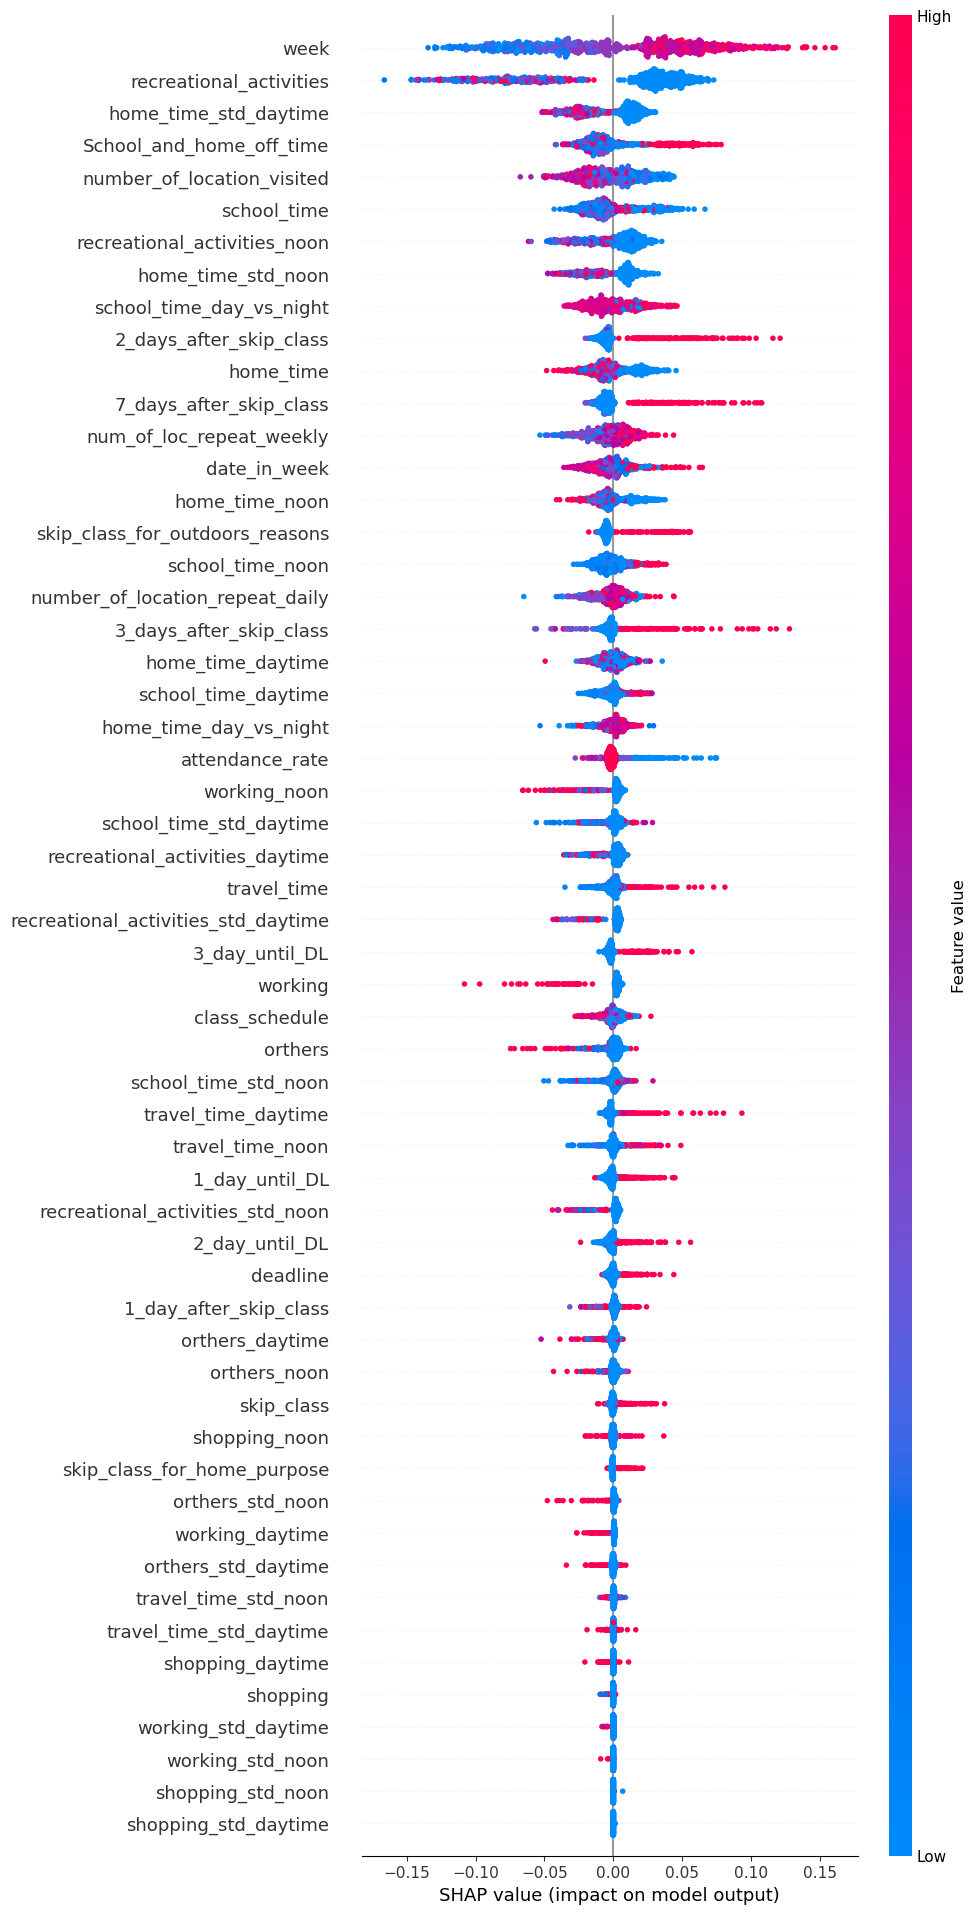
\includegraphics[width=0.45\linewidth,height=0.8\textheight]{Assets/FI_2_class.png}
}
% \caption{Random Forest}
% \label{fig_ShaplyRF}
% \end{subfigure}
% \hfill
% \begin{subfigure}[t]{0.24\textwidth}
\subfloat[Trường hợp 2\label{feat_imp3}]{
    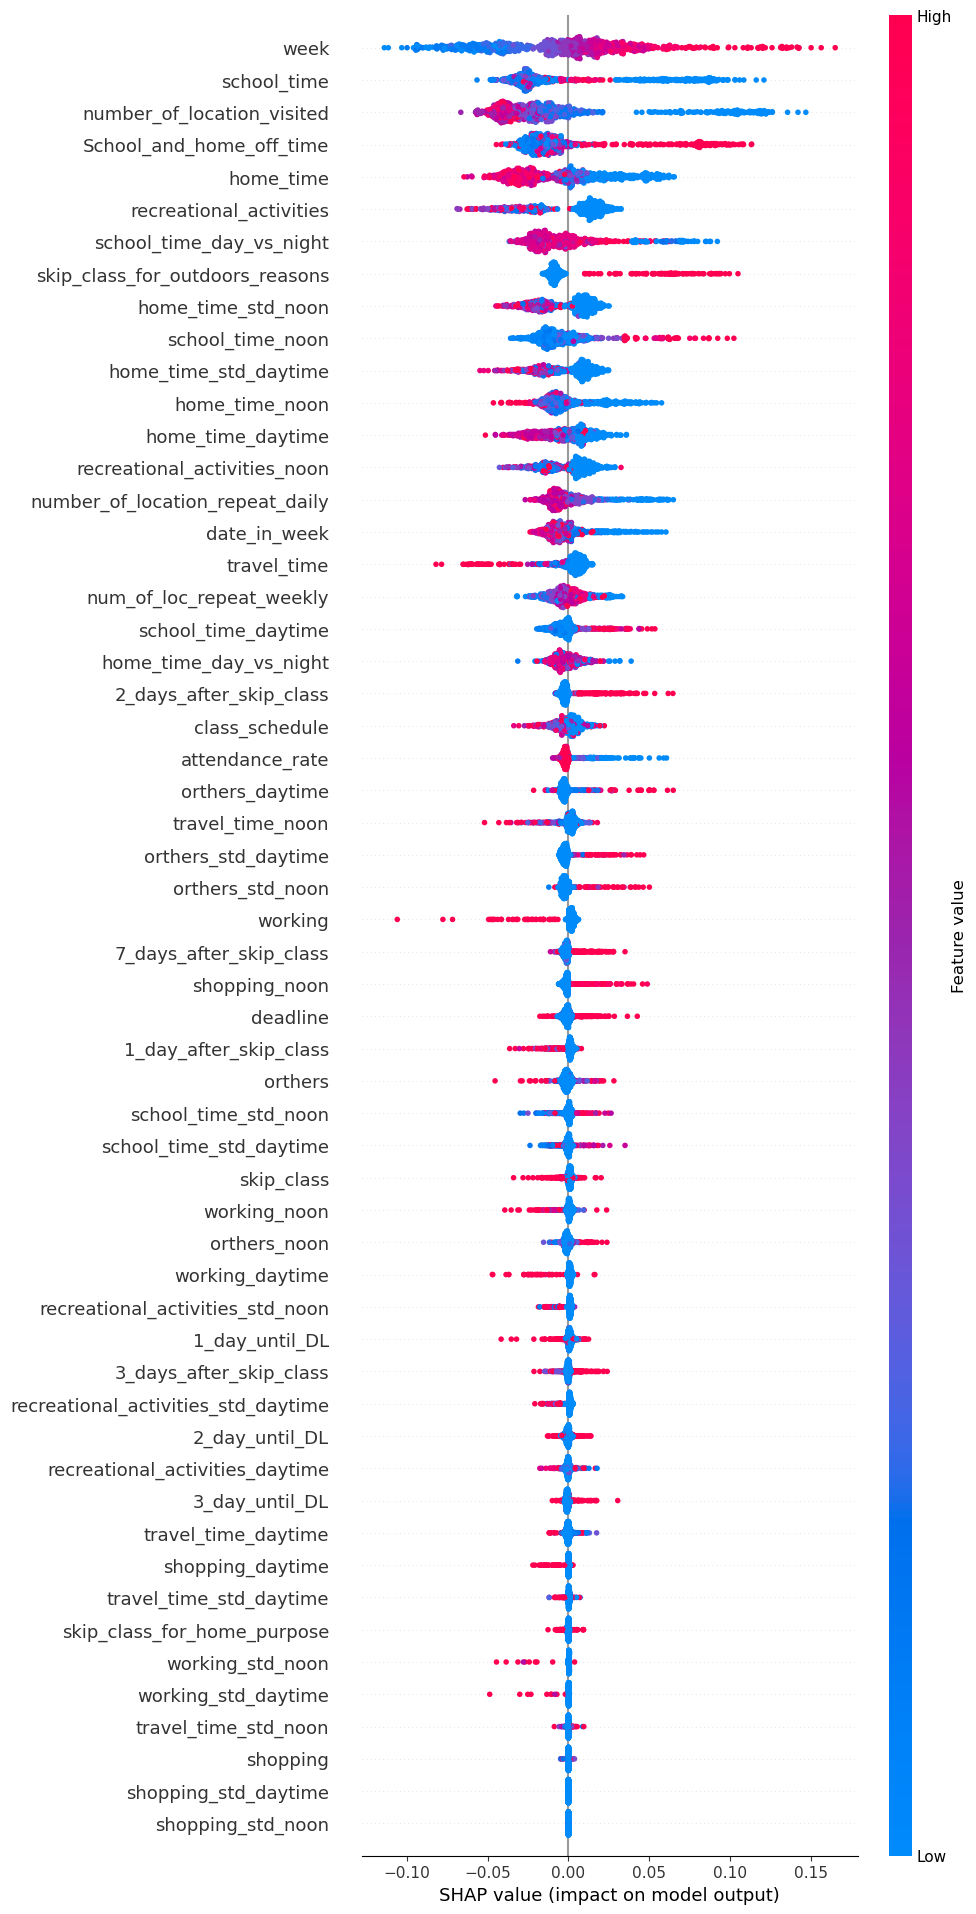
\includegraphics[width=0.45\linewidth,height=0.8\textheight]{Assets/FI_3_class.png}
}
% \caption{XGBoost model}
% \label{fig_ShaplyXG}
% \end{subfigure}
\caption{Biểu đồ phân tích đặc trưng bằng SHAP}
\label{feat_imp}
\end{figure}
% \section{Phân tích SHAP}

Với phân tích SHAP, tuần (week) là yếu tố gây nên căng thẳng tâm lý lớn nhất của sinh viên. Điều này khá dễ hiểu khi việc học diễn ra, càng về sâu của khoá học, lượng kiến thức càng nhiều và nâng cao, dẫn đến người học phải tốn nhiều thời gian hơn để nghiên cứu và hệ thống kiến thức. Điều này vô tình tạo áp lực lên sinh viên và dẫn đến căng thẳng tâm lý.

Một yếu tố khác có thể kể đến là thời gian giải trí (recreational activity) ảnh hưởng lớn đến sức khoẻ tinh thần của sinh viên. Với thời lượng giành cho các hoạt động giải trí cao, sinh viên sẽ có ít khả năng gặp phải các vấn đề tâm lý. Ngoài ra các yếu tố thời gian khác như thời gian ở nhà và ở trường (home time, và school time) cũng có ảnh hưởng lớn đến trạng thái sức khoẻ tinh thần của sinh viên.

Một yếu tố bổ sung mà tôi đã đề cập ở phần \ref{time_on_school_related_feature} là sự nghỉ học đóng góp tốt cho mô hình. Cụ thể hơn, với sinh viên nghỉ học đây có thể là dấu hiệu cho những vấn đề căng thẳng tâm lý, nhưng ngày sau ngày nghỉ học, các vấn đề đó sẽ phần nào được giải quyết (xem hình \ref{feat_imp}). Đây là một vấn đề đáng quan tâm khi là một bằng chứng chứng tỏ việc nghỉ học có thể giúp sinh viên giải quyết được các vấn đề tinh thần.


\section{Bàn luận}
Nghiên cứu này đã đề xuất phương pháp ứng dụng tín hiệu GPS liên tục từ điện thoại sinh viên trích xuất đặc trưng di chuyển và học tập của sinh viên mà vẫn đảm bảo tính bảo mật vị trí trong nghiên cứu sức khoẻ tinh thần dành cho sinh viên với độ chính xác cao (xấp xỉ 80\%) trong môi trường không kiểm soát. Đặc biệt hơn, nghiên cứu này cũng ứng dụng mới nhất trong lĩnh vực trí tuệ nhân tạo - XAI - trong việc khai phá tầm quan trọng của các đặc trưng trích xuất hiểu thêm sâu vào sức khoẻ tinh thần của sinh viên.

Việc phát triển hệ thống nhận diện sức khoẻ tinh thần trong tự nhiên đưa ra những yếu tố định lượng cho việc hiểu về sinh viên của người hoạt động giáo dục. Hơn thế việc có được các dữ liệu này có thể hỗ trợ nhà trường có thêm các cơ sở cho việc sắp xếp thời gian học tập giúp sinh viên có thể cân đối việc học và các việc cá nhân.

Tuy nhiên, nghiên cứu này chỉ có thể sử dụng dạng vị trí (nhà hàng, toà nhà, trường,...) để gán cho loại hoạt động của sinh viên (nhà, trường, giải trí,...). Việc này có thể vô tình gán sai hành động của sinh viên trong thực tế. Vì vậy, tôi đề xuất việc phát triển thêm phương pháp đánh giá hành động của con người hoặc ứng dụng trí tuệ nhân tạo tạo sinh để cải thiện việc hiểu hoạt động này rõ ràng hơn, từ đó chính xác hoá và giải quyết được cấc tình huống phức tạp trong hiện tại ví dụ nhận biết sinh viên đang làm gì trong một toà nhà đa chức năng (ăn uống, mua sắm, học tập).

Ngoài ra, nghiên cứu này đã đề cập các vấn đề liên quan đến vị trí, và hành vi của sinh viên song vẫn chưa hoàn thiện được các yếu tố xoay quanh cuộc sống của sinh viên hiện đại như thói quen tương tác xã hội, thời gian sử dụng điện thoại, học trực tuyến, ... Việc khai phá thêm đặc trưng này sẽ giúp mở rộng những đặc trưng cho việc chẩn đoán sức khoẻ tinh thần của sinh viên cũng như đưa được góc nhìn tổng quát hơn về sinh viên của mình.

\begin{figure}[!ht]
\subfloat[Không nghỉ học \label{feat_imb2}]{
    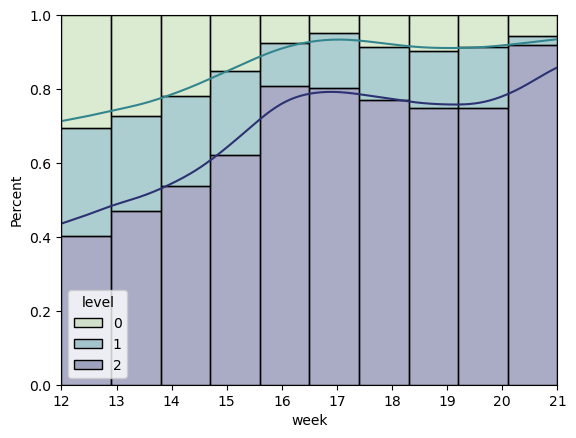
\includegraphics[width=0.45\linewidth]{Assets/not_skip_count.png}
}
% \caption{Random Forest}
% \label{fig_ShaplyRF}
% \end{subfigure}
% \hfill
% \begin{subfigure}[t]{0.24\textwidth}
\subfloat[Nghỉ học \label{feat_imb3}]{
    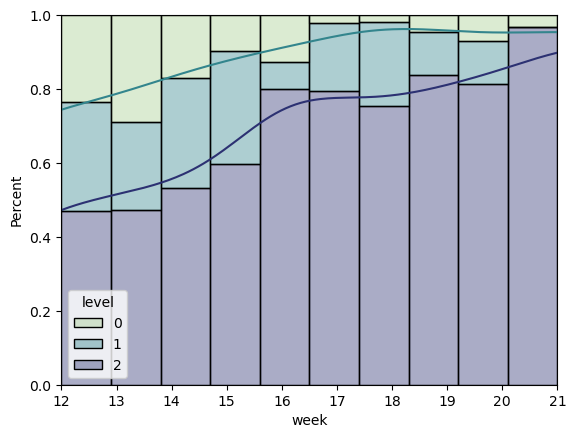
\includegraphics[width=0.45\linewidth]{Assets/skip_count.png}
}
% \caption{XGBoost model}
% \label{fig_ShaplyXG}
% \end{subfigure}
\caption{Biểu đồ tỉ số số lượng sinh viên theo trang thái tâm lý trong các tuần học đối với nhóm sinh viên có thực hiện (a) Không nghỉ học, (b) Nghỉ học trong ngày}
\label{feat_imp}
\end{figure}

Về các yếu tố học tập và thời gian, số lượng sinh viên bị căng thẳng cao có xu hướng chiếm phần lớn trong lượng sinh viên. Điều này là một vấn đề bình thường vì việc học thêm kiến thức hằng ngày tạo cho sinh viên áp lực khiến cho sinh viên có thể có những mệt mỏi dẫn đến căng thẳng. Ngoài ra, về số lượng sinh viên bị căng thẳng cao, hai nhóm sinh viên có nghỉ hocj và không nghỉ học có sự khác biệt lớn. Đối với nhóm nghỉ học, tỉ lệ sinh viên bị căng thẳng tăng đến tuần 16-17, tức tuần thi giữa kì, sau đó giữ nguyên. Còn đối với nhóm sinh viên còn lại, việc căng thẳng cao đạt đỉnh tại tuần 16-17. Điều này có thể do sinh viên đi học đầy đủ có điểm thi giữa kì tốt hơn và không chịu áp lực điểm thi cuối kì phải cao để qua môn còn với nhóm sinh viên nghỉ học phải chịu áp lực đó. Đặc biệt hơn, đối với sinh viên không nghỉ học, tỉ lệ sinh viên cảm thấy vui vẻ chiếm nhiều hơn so với nhóm sinh viên nghỉ học, thể hiện sinh viên đi học đầy đủ có thể phải chịu ít áp lực do học tập hơn nhóm còn lại. 

Một điều đáng quan tâm là yếu tố lý do cho sự nghỉ học. Về lý do nghỉ học cho các hoạt động bên ngoài, điều này là dấu hiệu của việc sinh viên bị căng thẳng tâm lý (hình \ref{feat_imp}). Để giải thích cho vấn đề này, việc sinh viên bị stress sẽ có xu hướng ra ngoài làm những việc thư giãn, điều này sẽ giúp cho sinh viên cảm thấy tốt hơn, dẫn đến những ngày có dữ liệu sinh viên nghỉ học để đi ra ngoài được gán với trạng thái tâm lý stress của sinh viên. Đặc biệt hơn việc nghỉ học để ở nhà lại có ít tác động đến sức khoẻ tinh thần của sinh viên hơn so với nghỉ học để cho các hoạt động bên ngoài. Theo tư duy thông thường, nhà là nơi để nghỉ ngơi và có thể là nơi để giải toả các vấn đề nhưng với cuộc sống sinh viên, thời gian ở nhà có thể được gán cho hai việc, nghỉ ngơi, hoặc hoàn thành các hạn nộp bài. Hai yếu tố này diễn ra trong cùng một loại vị trí và có tác động trái ngược nhau, vì vậy việc nghỉ học để ở nhà được phân tích gây nên yếu tố ở nhà có thể ảnh hưởng tích cực lẫn tiêu cực đến sức khoẻ tinh thần của sinh viên

\begin{figure}[!ht]
    \centering
    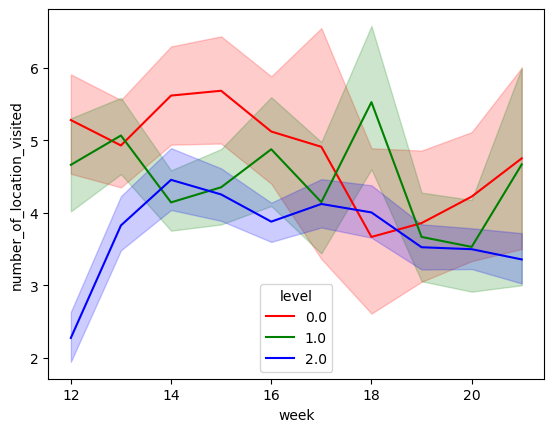
\includegraphics[width=0.75\linewidth]{num_of_loc_by_week.png}
    \caption{Biểu đồ biểu diễn số lượng địa điểm đến của sinh viên theo tuần chia theo mức độ căng thẳng}
    \label{num_of_loc_week}
\end{figure}

\begin{figure}[!ht]
    \centering
    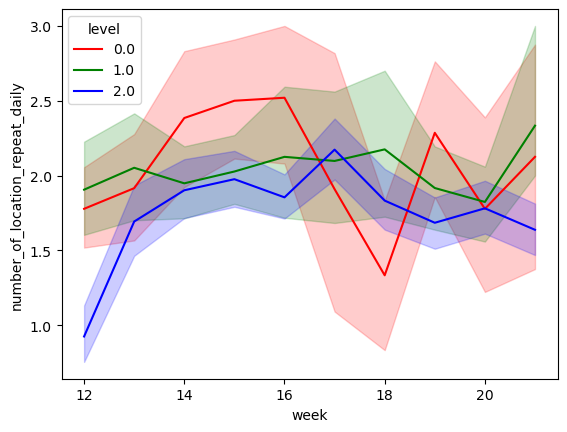
\includegraphics[width=0.75\linewidth]{num_of_location_daily_week.png}
    \caption{Biểu đồ biểu diễn số lượng địa điểm lặp lại trong 2 ngày liên tiếp của sinh viên theo tuần chia theo mức độ căng thẳng}
    \label{daily repeat}
\end{figure}

Một điều đáng chú ý khác là thói quen di chuyển của sinh viên. Phân tích đặc trưng chỉ ra rằng số lượng điểm đến ảnh hưởng tích cực với trạng thái của sinh viên. Lấy ví dụ một sinh viên có số lượng địa điểm đến trong một ngày thấp, điều này có thể chỉ ra người này chỉ làm việc trong một không gian nhất định, việc thiếu sự đổi mới sẽ có thể dẫn đến việc thiếu giao tiếp và dẫn đến stress. Ngược lại, nếu một người được ghi nhận ở nhiều địa điểm, điều này chứng tỏ người ấy đã di chuyển nhiều, và việc di chuyển sẽ giúp người đó có các tương tác xã hội, góp phần làm giảm căng thẳng tâm lý. 

Đặc biệt hơn, về yếu tố độ lặp lại của các trạng thái, sự lặp đi lặp lại theo hai ngày liên tục hoặc một ngày của hai tuần liên tiếp đạt giá trị vừa phải có thể là dấu hiệu người đó đang có trạng thái tâm lý thoải mái. Việc này có thể lý giải bằng hành vi của con người khi con người ta có nhiều sự lựa chọn, con người thường sẽ lựa chọn trải nghiệm, dẫn đến sự lặp lại giảm xuống. 

Đối chiểu với kết quả của nghiên cứu này, với nhóm sinh viên bị căng thẳng tâm lý nặng, nhóm sinh viên này có xu hướng di chuyển đến các địa điểm ít hơn so với các sinh viên khác (hình \ref{num_of_loc_week}). Ngoài ra nhóm này cũng ít khi thay đổi những điểm đến của mình (hình \ref{daily repeat}). Điều này vô hình làm cho sinh viên thiếu sự thay đổi trong các hoạt động trong ngày dẫn đến các vấn đề tinh thần như đã trình bày ở trên.


\begin{figure}[!ht]
    \centering
    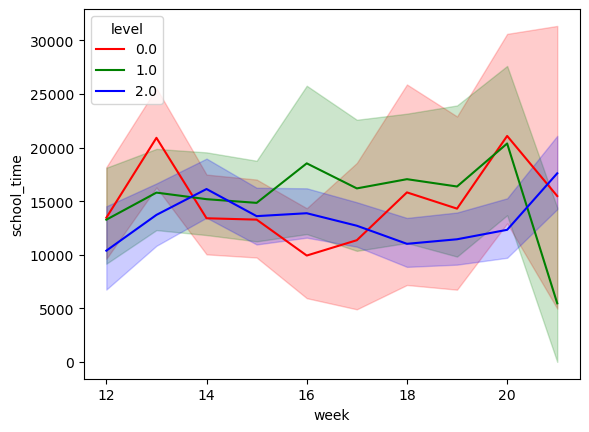
\includegraphics[width=0.75\linewidth]{Shooltime_week_line.png}
    \caption{Biểu đồ biểu diễn thời gian đi học của sinh viên theo tuần chia theo mức độ căng thẳng}
    \label{line_week_school}
\end{figure}
Ngoài ra, việc các thời gian giành cho các địa điểm cũng mang ý nghĩa nhất định đến việc căng thẳng tâm lý của sinh viên. Một ví dụ điển hình ở đây là phân tích về thời gian đi học. Thời gian đi học là một phần quan trọng với sinh viên khi đây là cơ hội để các sinh gặp được những người bạn, giáo sư của họ. Việc gặp gỡ và giao tiếp xã hội sẽ giúp cho các sinh viên giải toả được áp lực, từ đó sinh viên có thể cảm thấy tốt hơn. Cụ thể trong nghiên cứu này, hình \ref{line_week_school} đã thể hiện những sinh viên bị stress có xu hướng ở trường ít hơn sinh viên không bị căng thẳng tâm lý. Ngoài ra với nhhoms căng thẳng cao, nhóm này thường có thời gian đi học thấp nhất. Vì vậy có thể nhận thấy một mối tương quan giữa thời gian đi học và sức khoẻ tâm lý của sinh viên.

\begin{figure}[!ht]
    \centering
    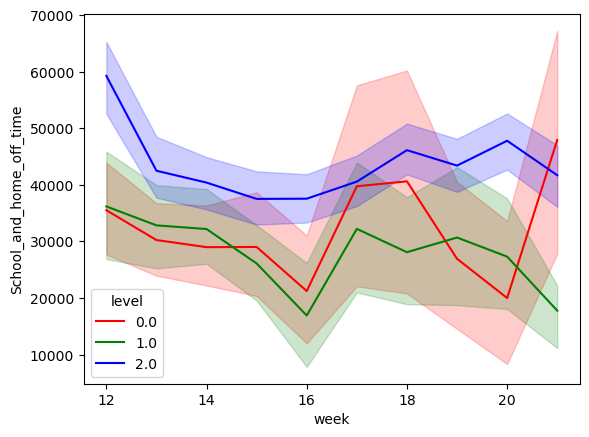
\includegraphics[width=0.75\linewidth]{line_week_home_a_school_off.png}
    \caption{Biểu đồ biểu diễn thời gian ở ngoài nhà và trường của sinh viên theo tuần chia theo mức độ căng thẳng}
    \label{line_week_homeaschooloff}
\end{figure}

Hơn thế, thời gian ngoài nhà và lớp học cũng đáng được quan tâm. Với thời gian này quá nhiều có thể gây nên những căng thẳng tâm lý. Như trong nghiên cứu này sinh viên gặp tình trạng căng thẳng cao (đường màu xanh dương hình \ref{line_week_homeaschooloff}) có thời gian ở ngoài nhà và trường nhiều nhất. Để lý giải vấn đề này, thời gian ở ngoài nhà và lớp học phản ánh khoảng thời gian sinh viên phải ở bên ngoài. Nếu sinh viên ở bên ngoài lâu, việc này sẽ làm mất cân bằng cuộc sống của sinh viên, và khi sinh viên này nhận ra còn việc làm ở nhà và ở trường sẽ gây ra trạng thái căng thẳng.


Vì vậy các yếu tố hành động, và các yếu tố hành vi khai thác từ hành động chứng minh được ý nghĩa trong việc đặc trưng cho cách mà sinh viên đối mặt với căng thẳng từ đó ta có thể lợi dụng điểm này để khai thác tạo nên các ứng dụng nhận diện sức khoẻ tinh thần dành cho sinh viên.


